\documentclass[12pt, a4paper, lithuanian]{article}

\usepackage[utf8x]{inputenc}
\def\LTfontencoding{L7x}
\usepackage[\LTfontencoding]{fontenc}
\usepackage[lithuanian]{babel}
\usepackage{amsmath}

\usepackage{VUMIF}
\usepackage{listings}
\usepackage{graphicx}

% "define" Scala
\lstdefinelanguage{scala}{
  morekeywords={abstract,case,catch,class,def,%
    do,else,extends,false,final,finally,%
    for,if,implicit,import,match,mixin,%
    new,null,object,override,package,%
    private,protected,requires,return,sealed,%
    super,this,throw,trait,true,try,%
    type,val,var,while,with,yield},
  otherkeywords={=>,<-,<\%,<:,>:,\#,@},
  sensitive=true,
  morecomment=[l]{//},
  morecomment=[n]{/*}{*/},
  morestring=[b]",
  morestring=[b]',
  morestring=[b]""
}

\usepackage{color}
\definecolor{dkgreen}{rgb}{0,0.6,0}
\definecolor{gray}{rgb}{0.5,0.5,0.5}
\definecolor{mauve}{rgb}{0.58,0,0.82}


% Default settings for code listings
\lstset{frame=tb,
  language=scala,
  captionpos=b,
  aboveskip=3mm,
  belowskip=3mm,
  showstringspaces=false,
  columns=flexible,
  basicstyle={\small\ttfamily},
  numbers=none,
  numberstyle=\tiny\color{gray},
  %keywordstyle=\color{blue},
  %commentstyle=\color{dkgreen},
  %stringstyle=\color{mauve},
  frame=single,
  breaklines=true,
  breakatwhitespace=true
  tabsize=3
}

\renewcommand{\lstlistingname}{Kodo pavyzdys}

% \usepackage[mathcsdepttitle]{VUMIF} % --- matematinės informatikos katedros
%     titulinio puslapio formatavimas

% Titulinio puslapio reikalai
\vumifdept{Informatikos katedra}
\vumifpaper{Mokslo tiriamasis darbas}
\title{Funkcinio-reaktyvaus programavimo taikymas įvykių kaupimo sistemose}
\engtitle{Functional Reactive Programming in Event Sourcing Systems}
\author{
    1 kurso 12 grupės studentas \\
    Žilvinas Kučinskas
}

\supervisor{Viačeslav Pozdniakov}
\reviewer{prof. Rimantas Vaicekauskas}
\date{Vilnius \\ 2014}

\begin{document}

\maketitle

\tableofcontents

\section{Magistro darbo objekto apžvalga bei tyrimo problemos aprašymas}
\subsection{Tyrimo objektas}

    Tyrimo objektas yra funkcinio-reaktyvaus programavimo bei įvykių kaupimo principai.

\subsection{Darbo tikslai ir uždaviniai}

    Darbo tikslas yra pritaikyti funkcinio-reaktyvaus programavimo principus įvykių kaupimo sistemose taip, jog būtų išpildyti šie reikalavimai:

\begin{itemize}

    \item įvykių kaupimo sistemos skaitymo modelis būtų be būsenos;

    \item įvykių kaupimo sistemos skaitymo modelis būtų kuriamas tik per įvykių kompoziciją;

    \item įvykių kaupimo sistemos skaitymo modelio programinis kodas būtų griežtai tipizuotas.

\end{itemize}

    Siekiant šio tikslo, turi būti išspręsti šie uždaviniai:

\begin{itemize}
        \item įrodyti, kad funkcinį-reaktyvų programavimą įmanoma taikyti įvykių
            kaupimo sistemose;
        \item sukurti konkretizuotą kalbą (angl. domain specific language), apjungiančią funkcinio-reaktyvaus programavimo
            bei įvykių kaupimo principus;
        \item aprašyti konkretizuotuos kalbos kūrimo metodiką, apibrėžti gautų rezultatų apribojimus, suformuluoti iškilusias problemas bei paaiškinti jų priežastis.
\end{itemize}

\subsection{Tyrimo aktualumas}

    Funkcinis reaktyvus programavimas integruoja laiko tėkmę bei sudėtinius įvykius į funkcinį programavimą. Šis principas suteikia elegantišką būdą išreikšti skaičiavimus interaktyvių animacijų, robotikos, kompiuterinio vaizdavimo, vartotojo sąsajos ir modeliavimo srityse \cite[p. 4]{ELM:FRP}. Pagrindinės funkcinio reaktyvaus programavimo sąvokos:

\begin{itemize}
        \item signalai arba elgsena - reikšmės, besikeičiančios bėgant laikui;
        \item įvykiai - momentinių reikšmių kolekcijos arba laiko-reikšmės poros.
\end{itemize}

    Funkcinis-reaktyvus programavimas įgalina apsirašyti elgseną deklaratyviai \cite[p.1]{ElliottHudak97:Fran}. Elgsena ir įvykiai gali būti komponuojami kartu, išreikšti vienas per kitą. Funkcinis reaktyvus programavimas apibrėžia kaip signalai arba elgsena reaguoja į įvykius. \cite[p. 1]{Survey} Šį principą galima iliustruoti pavyzdžiu. Tarkime turime Excel lapą, kuriame yra trys laukai: darbuotojo pradirbtos valandos, valandinis užmokestis bei formulė, kuri paskaičiuoja konkretų darbuotojo atlyginimą. Darbuotojui pradirbus daugiau valandų, atnaujinamas pradirbtų valandų skaičius. Kartu atsinaujina ir pačios formulės reikšmė, tai yra konkretus užmokestis pakinta. Šiuo atveju įvykus reikšmės atnaujinimo įvykiui, nuo jos priklausomos formulės taipogi atsinaujina arba tam tikras įvykis iššaukia elgseną sistemoje.

    Įvykių kaupimo principo esmė – objektas yra atvaizduojamas kaip įvykių seka. Kaip pavyzdį tai galima parodyti remiantis banko sąskaita. Tarkime vartotojas, banko klientas, turi 100 litų sąskaitos balansą. Tarkime vartotojas nusipirko prekę už 20 litų, tada įnešė į savo sąskaitą 15 litų ir galiausiai nusipirko tam tikrą paslaugą už 30 litų. Akivaizdu, jog turint šią įvykių seką, galima atvaizduoti dabartinę objekto būseną - tai yra 65 litai vartotojo sąskaitoje. Įvykių kaupimo principas užtikrina, jog visi būsenos pasikeitimai yra saugomi įvykių žurnale kaip įvykų seka \cite{vernon2013implementing}. Įvykių kaupimo principui yra būdinga, jog įvykių negalimą ištrinti bei atnaujinti, duomenys yra nekeičiami, dėl to įvykių žurnalas yra sistemos gyvavimo istorija (tiesos šaltinis). Tačiau toks modelis turi ir trūkumų. Jis nėra pritaikytas patogiam užklausų rašymui. Iš įvykių srautų yra kuriamos projekcijos, skirtos konkretiems sistemoms poreikiams, pavyzdžiui: paieškai, klasifikacijai ar ataskaitų ruošimui.

    Pritaikius funkcinį-reaktyvų programavimą įvykių kaupimo principu paremtose sistemose būtų galima modeliuoti ne tik momentinius įvykius, tačiau turėti ir jų istoriją. Yra poreikis sukurti konkretizuotą kalbą (angl. domain specific language), kuri įgalintų paslėpti įvykių žurnalą (arba duomenų saugyklą). Pastarosios naudotojas galėtų orientuotis į pačią sprendžiamos srities problemą, nekreipdamas dėmesio į žemesnio lygio realizacijos detales. Šiuo atveju vbūtų galima deklaratyviai (ką kažkuri programos dalis turi daryti) apsirašyti elgseną, nutikus įvykiui, kartu su imperatyviomis(instrukcijos, kurios aprašo, kaip programos dalys atlieka savo užduotis) struktūromis.

\subsection{Pritaikymo pavyzdys}

    Tarkime turime domeno sritį - bankininkystė. Turime įvykių srautą - vartotojų sukūrimas. Naudojant įsivaizduojamą Scala API galima sukurti vartotojų paieškos puslapį pagal vardą ir pavardę. Demonstacija pateikta \ref{creation} kodo pavyzdyje.

\begin{lstlisting}[caption=- vartotojų paieškos puslapis naudojant įsivaizduojamą Scala API, label=creation]
// stream model
case class CustomerCreate (val name: String, val surname: String, val personalNum: String)

val es = EventSourceConnection(url)
val createStream = Stream(es, "customerCreate")

class case CustomerModel(val name: String, val surname: String, val personalNum: String)  extends ViewableModel

trait CustomerArgModel extends Arg2Model[String,String]{
  val name: Option[String]
  val surname: Option[String]
}

//args are passed on form view/post
val customerView = View(args: CustomerArgModel).foldLeft(
  (acc,event) => event match {
    case CustomerCreate(name, surname, personalNum) =>
      for {
        newName <- name
        newSurname <- surname
        newPersNum <- personalNum
        if (args.name == name && args.surname == surname)
      } yield CustomerModel(newName, newSur, newPersNum)
  }
)
// getting data for all Kucinskai
val specificData = customerView(None, Some("Kucinskas")): Option[List[CustomerModel]]
\end{lstlisting}

    Šiuo atveju veiksmai peržiūrint duomenis yra sumaišomi kartu su veiksmais gaunant įvykius. Verta pastebėti, jog lokali duomenų saugykla nebuvo paminėta arba apibrėžta. Pastaroji gali būti sugeneruota bei valdoma automatiškai.

    Antruoju pavyzdiniu atveju turimas vartotojo balanso(įplaukiančios/išplaukiančios lėšos) įvykių srautas ir norima gauti vartotojo, kurio asmens kodas yra \emph{39008226547}, einamosios savaitės sąskaitos balansą. Demonstacija pateikta \ref{balance} kodo pavyzdyje.

\begin{lstlisting}[caption=- vartotojo einamosios sąskaitos balansas naudojant įsivaizduojamą Scala API, label=balance]
val duration = 1.weeks
val personalNum = "39008226547"
val balanceStream = Stream(es, "customerBalance")
val notOlderThanOneWeek =
    for {
        event <- balanceStream
        filtered <- event.filter(_.personalNum == personalNum
            && (DateTime.now - _.timeStamp) >= duration)
    } yield filtered
val sum = notOlderThanOneWeek.toList.sum
\end{lstlisting}

    Šiuo atveju \emph{event} kintamasis yra galimai įvykių srauto monada (terminas vartojamas funkciniame programavime, kilęs iš kategorijų teorijos ir turi savas taisykles), o \emph{filtered} kintamasis - duomenų saugyklos monada. Bendruoju atveju skirtingos monados tarpusavyje nesiderina \cite{DBLP:conf/fp/KingW92}. Dėl to reikia išsiaiškinti - ar yra įmanoma ir kaip šias monadas suderinti.

\subsection{Tyrimo metodika}

    Darbo tikslui pasiekti tiriamojoje dalyje bus pasirinkta konkreti funkcinė programavimo kalba (pvz.: Haskell, Scala) bei aprašoma kūrimo metodika.

\subsection{Laukiami rezultatai}

    Magistrinio darbo metu planuojama išnagrinėti funkcinio-reaktyvaus programavimo ir įvykio kaupimo principus, įrodyti, jog šie principai gali būti panaudoti kartu bei suderinti, sukurti konkretizuotą kalbą (angl. domain specific language), apjungiančią šiuos principus, bei aprašyti kūrimo eigos metodiką, apibrėžti gautus rezultatus, suformuluoti apribojimus, iškilusias problemas bei paaiškinti jų priežastis.

\section{Literatūros analizė}
\subsection{Funkcinis-reaktyvus programavimas}

Daugiausia remtąsi \cite{Survey}.

\subsubsection{Įvadas}

Funkcinis-reaktyvus programavimas, toliau vadinamas tiesiog FRP, yra būdas modeliuoti reaktyvų - besikeičiančius laiko tekmėje bei reaguojančius į išorinį stimulą - elgesį visiškai funkcinėse programavimo kalbose. FRP leidžia deklaratyviu ir paprastu būdu modeliuoti sistemas, kurios turi reaguoti į duomenis bėgant laikui.

\subsubsection{Pagrindinis tiklas}

Pagrindinis funkcinio-reaktyvaus programavimo tikslas:

\begin{itemize}

	\item saugus programavimas - kompiliatorius turi kiek įmanoma patikrinti programų korektiškumą;

	\item efektyvus programavimas - programos turėtų veikti realiu laiku, todėl efektyvios ir optimizuotos operacijos yra būtinos;

	\item komponavimas - FRP leidžia kurti programas iš smulkesnių programų, o ne orientuotą į problemą, vientisą kodą.

\end{itemize}

\subsubsection{Sąvokos}

Pagrindinės FRP sąvokos yra:

\begin{itemize}

	\item signalai arba elgsena - besikeičiančios laike reikšmės;

	\item įvykiai - kolekcija momentinių reikšmių arba laiko-reikšmės poros.

\end{itemize}

FRP pasiekia reaktyvumą naudodamas konstrukcijas, kurios tiksliai apibrėžia kaip signalai arba elgsena pasikeičia reaguodami į įvykius. Tai yra pagrindinis būdas išreiškiant bei realizuojant elgseną. Kitu būdu, elgsena gali būti laiko semantinės funkcijos\footnote{http://msdl.cs.mcgill.ca/people/tfeng/docs/as/node5.html}, kuriose laikas yra pakeičiamas kilus įvykiui.

\subsubsection{Sąvybės}

Anot anksčiausios funkcinio-reaktyvaus programavimo formuluotės \cite{ElliottHudak97:Fran}, pagrindinės sąvybės, kuriomis pasižymi FRP:

\begin{itemize}

	\item elgsenos arba singalų modeliavimas bėgant laikui,

	\item įvykių, kurie turi baigtinį skaičių atsitikimų daugelyje laiko taškų, modeliavimas,

	\item perjungimas (angl. switching) - sistema gali pasikeisti dėl atsitikusių įvykių,

	\item analizės detalių, tokių kaip reaktyvaus modelio įvykių ėmimo dažnis, atskyrimas.

\end{itemize}

\subsubsection{Įvykių srautas}

Pagal \cite{Bass:2007:Mythbusters}, įvykių srautas yra eilė pagal laiką surikiuotų įvykių, pavyzdžiui akcijų rinkos srautas.

Įvykių srautas kaip duomenų srauto tipas formaliai atrodo kaip pora (s, t), kur s yra seka surikiuotų sąrašo įvykių, o t yra seka laiko intervalų ir kiekvienas intervalas yra netuščias.

Tokio duomenų srauto pavyzdžiai gali būti:

\begin{itemize}

	\item akcijų kursas,

	\item paspaudimų srautas,

	\item tinklo srautas,

	\item GPS\footnote{http://en.wikipedia.org/wiki/Global\_Positioning\_System} duomenys.

\end{itemize}

Įvykių srauto apdorojimas pagal atsitikimo laiką turi privalumų:

\begin{itemize}

	\item įvykių apdorojimo algoritmai naudoja mažai atminties, nes jiems nereikia prisiminti daug įvykių;

	\item algoritmai gali būti labai greiti;

	\item gavus įvykį, skaičiavimai atliekami iškart, todėl galima perduoti rezultatą kitam skaičiavimui ir pamiršti įvykį.

\end{itemize}

Įvykių srauto apdorojimas labiau akcentuoja didelio našumo duomenų gavimą ir matematinių algoritmų pritaikymą įvykių duomenims. Taip pat įvykių srautai įprastai pritaikomi konkrečiai sistemai ar organizacijai.

\subsubsection{Įvykių srautas funkciniame programavime}

Vietoje įvykių srauto, galima naudoti klausytojo projektavimo šabloną \cite{WhiteboardPattern}, tačiau ilgame programinės įrangos kūrimo gyvavimo cikle įvykių srauto naudojimas palengvina kai kuriuos dalykus. Pavyzdžiui, imperatyvaus programavimo atžvilgiu, viename metode turime klausytoją, kuris reaguoją į situaciją /textit{A}, tačiau iškilus situacijai /textit{B}, šis klausytojas yra pašalinamas. Šiuo atveju programinis kodas, kuris valdo klausytojo gyvavimo ciklą yra įsipynęs keliose skirtingose kodo vietose, ko pasekoje tai reiškia, jog yra sunkiau palaikyti, stebėti, keisti bei suprasti šias vietas. Abstrahuojant klausytojų gyvavimo ciklo valdymo idėją tampa lengviau programuoti pagal tai kas turėtų nutikti, o ne pagal tai, ką kompiuteris turėtų daryti toliau. Tačiau turbūt didesnis įvykių srauto pranašumas yra tai, jog pastarasis gali būti transformuojamas ir komponuojamas. Toliau bus aprašomi operacijos arba veiksmai bei sutrumpinti išeities kodo pavyzdžiai, kuriuos galima atlikti su įvykių srautu remiantis Reactive Web\footnote{http://scalareactive.org} karkasu, skirtu Scala\footnote{http://www.scala-lang.org} programavimo kalbai.

Pirmas veiksmas - įvykio srauto sukūrimas. Jis pavaizduotas \ref{creation} kodo pavyzdyje.  Pirmiausia sukuriamas įvykių šaltinis, kuris po to priskiriamas įvykių srautui.

\begin{lstlisting}[caption=- įvykių srauto sukūrimas, label=creation]
	val eventSource = new EventSource[String]{}
	scheduleTask(10000) {
		eventSource.fire("Event after 10 seconds")
	}

	val eventStream: EventStream[String] = eventSource
\end{lstlisting}

Taip pat \textit{EventSource} (įvykių šaltinis) turi naudingą poklasį \textit{Timer} (laikrodis). Jo realizacija pavaizduota \ref{timer} kodo pavyzdyje. Šis sukuria tiksėjimo įvykius duotu laiko intervalu.

\begin{lstlisting}[caption=- įvykių srauto sukūrimas, label=timer]
	val timer = new Timer(0, 2000, {t =>  t >= 32000})

	for(t <- timer)
    	yield "timer: " + t.toString
\end{lstlisting}

Įvykių srautas valdo kolekciją klausytojų, tačiau konceptualiai reikėtų mąstyti kitaip. Klausytojo pridėjimas iš tikrųjų reiškia funkcijos iškvietimą kiekvienam kilusiui įvykiui, kitais žodžiais kiekvienam įvykių srauto įvykiui. Lygiai taip pat kaip Scala programavimo kalboje norint įvykdyti funkciją kiekvienai kolekcijos reikšmei yra iškviečiama \textit{foreach} funkcija. Tačiau įvykių srauto atveju, \textit{foreach} grąžina rezultatą akimirksniu, o funkcija yra išsaugoma ir vėliau įvykdoma kai tik gaunamas koks nors įvykis. Šio atvejo praktinis variantas pademonstruotas \ref{foreach} kodo pavyzdyje.

\begin{lstlisting}[caption=- klausytojų pridėjimas, label=foreach]
	val eventSource = new EventSource[String] {}
	  
	// The following is syntactic sugar for
	// eventSource.foreach(event => alert("You fired: '" + event + "'"))
	for(event <- eventSource) {
	 	alert("You fired: '" + event + "'")
	}

\end{lstlisting}

Rinkinys transformacijų metodų įvykių srautą padaro labai universaliu. Šios transformacijos grąžina modifikuotą įvykių srautą. Transformacijas galima atlikti viena po kitos. Tai primena transformacijas galimas su Scala kolekcijomis, pavyzdžiui \ref{collectionTransformation} kodo pavyzdyje. Kai tik originalus įvykių srautas gauna įvykį, transformuotas įvykių srautas gauna savo įvykį pritaikant klausytojo funkciją.

\begin{lstlisting}[caption=- kolekcijos transformacijos, label=collectionTransformation]
	List(1,2,3).map(_ * 10).filter(_ < 25)
\end{lstlisting}

Jeigu įvykių srautas gauna labai daug įvykių, tačiau aktualūs yra tik dalis jų, galima naudoti filtravimą, tai yra \textit{filter} metodą. Tai demonstruojama \ref{filter} kodo pavyzdyje. Čia kiekvienam įvykiui yra pritaikomas predikatas. Jeigu jis įvertinimas kaip teisingas arba kitaip \textit{true}, įvykis yra gaunamas transformuotame įvykių sraute.

\begin{lstlisting}[caption=- įvykių srauto filtravimas, label=filter]
	val eventSource = new EventSource[String] {}
	eventSource.filter(_.length < 5)
\end{lstlisting}

Kitas esminis kolekcijų metodas yra \textit{map}. Jis leidžia transformuoti kolekciją pritaikant tam tikrą funkciją kiekvienam kolekcijos elementui. Pritaikius yra grąžinama nauja modifikuota kolekcija. Lygiai taip pat šis metodas gali būti pritaikytas įvykių srautui. Šis atvejis demonstruojamas \ref{map} kodo pavyzdyje. 

\begin{lstlisting}[caption=- įvykių visiškas transformavimas, label=map]
	val eventSource = new EventSource[String] {}
	eventSource.map(_.reverse)
\end{lstlisting}


\subsection{Įvykių kaupimas}

Šiame skyriuje yra aprašomos žinios apie įvykių kaupimą, pliusus ir minusus, įvykių srautus bei įvykių kaupimą funkciniame programavime remiantis Vaughn Vernon surinkta ir aprašyta informacija \cite{vernon2013implementing}.

\subsubsection{Įvadas}

Kartais verslui svarbu fiksuoti objekto pasikeitimus domeno modelyje\footnote{http://en.wikipedia.org/wiki/Domain\_model}. Šiuos pasikeitimus galima stebėti skirtingais būdais. Įprastai yra pasirenkama stebėti kai esybė\footnote{http://en.wikipedia.org/wiki/Entity} yra:

\begin{itemize}

	\item sukurta,

	\item paskutinį kartą modifikuota

	\item bei kas atliko modifikaciją.

\end{itemize}

Tačiau šis būdas nepateikia jokios informacijos apie vienkartinius pasikeitimus.

Atsiradus poreikiu stebėti pasikeitimus detaliau, verslas reikalauja dar daugiau metaduomenenų\footnote{http://en.wikipedia.org/wiki/Metadata}, ko pasekoje tokie faktai kaip individualios operacijos laiko tekmėje bei jų įvykdymo laikas tampa svarbūs. Šie poreikiai verčia įvesti audito žurnalą fiksuoti labai tikslias panaudojimo atvejų metrikas, tačiau pastarasis būdas turi apribojimų. Jis gali atskleisti dalį informacijos apie tai kas nutiko sistemoje, leisti rasti bei ištaisyti dalį riktų bei klaidų programinėje įrangoje, bet audito žurnalas neleidžia patikrinti domeno objekto būsenos prieš ir po tam tikrų pasikeitimų. O jeigu būtų galima išgauti daugiau informacijos iš pasikeitimų stebėjimo?

Visi programinės įrangos kūrėjai susiduria su labai tiksliu pasikeitimų stebėjimu. Įprastas ir populiarus pavyzdys yra išeities kodo saugyklos, tokios kaip CVS\footnote{http://www.nongnu.org/cvs/}, Subversion\footnote{http://subversion.apache.org/}, Git\footnote{http://git-scm.com/} arba Mercurial\footnote{http://mercurial.selenic.com/}. Visos šios pataisų valdymo sistemos leidžia stebėti pirminių failų pasikeitimus. Įrankiai leidžia peržiūrėti išeities kodo artefaktus nuo pačios pirmosios pataisos iki paskutinės. Kai visi išeities failai yra nusiunčiami į pataisų kontrolės sistemą, ši gali stebėti pasikeitimus viso programinės įrangos kūrimo gyvavimo ciklo metu.

Jeigu šis principas būtų pritaikytas vienai esybei, tada vienam agregatui\footnote{http://martinfowler.com/bliki/DDD\_Aggregate.html} bei galiausiai kiekvienam modelio agregatui, galima suprasti kokią naudą atneša sistemos objektų pasikeitimų stebėjimas:

\begin{itemize}

	\item Kas būtent nutiko modelyje, jog agregato egzempliorius buvo sukurtas?

	\item Kas nutiko agregato egzemplioriui bėgant laikui? (Operacijų požiūriu)

\end{itemize}

Turint visų atliktų operacijų istoriją, galima palaikyti laikinus modelius. Toks kaitos stebėjimas yra įvykių kaupimo principas. \ref{pic:es} diagramoje pateika šio principo aukšto lygio reprezentacija. Agregatai publikuoja įvykius, kurie yra išsaugomi įvykių saugykloje ir naudojami sekti modelio būsenos pasikeitimus. Verta paminėti, jog įvykiai reprezentuoja tam tikrą būsenos pasikeitimą bėgant laikui, todėl jie nėra atnaujinami arba ištrinami. Saugykla nuskaito įvykius iš įvykių saugyklos ir pritaiko juos vieną po kito taip atkurdama agregato būseną. 

\begin{figure}[ht]
	\centering
	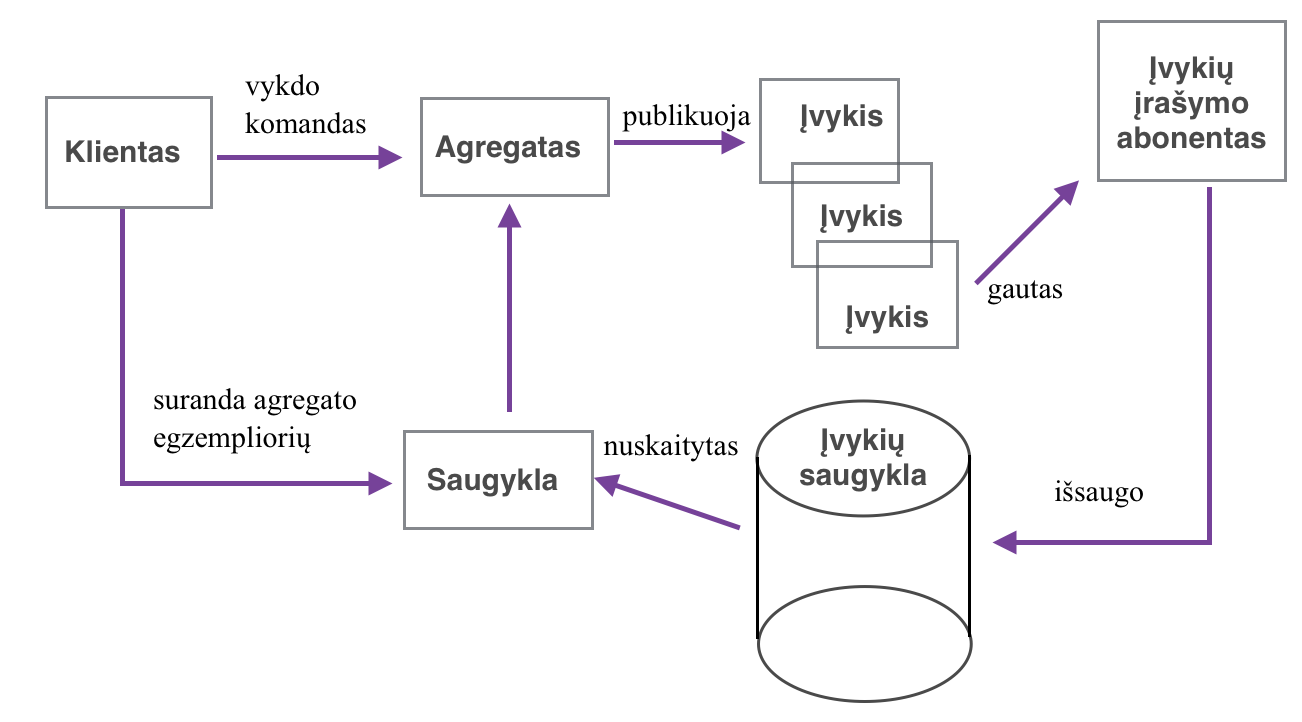
\includegraphics[width=0.9\linewidth]{pics/es.png}
	\caption{Įvykių kaupimo aukšo lygio reprezentacija}
	\label{pic:es}
\end{figure}

\subsubsection{Momentinė kopija}

Ilgame periode sistemoje susikaupia daugybė įvykių. Atkuriant agregato būseną reikia atkartoti šimtus, tūkstančius ar net milijonus įvykių. Tai tampa šio modelio silpnąja puse, nes įvykių atkartojimas užtrunka vis ilgiau sistemai plečiantis.

Tačiau šio duomenų kamsčio galima išvengti naudojant agregato būsenos momentines kopijas. Tam tikrame įvykių saugyklos istorijos taške yra padaroma agregato būsenos kopija. Serializuota agregato būsena yra įrašoma į įvykių saugyklą. Nuo to momento, agregatas yra atkuriamas pirmiausia naudojantis naujausia jo būsenos momentine kopija ir tik po to atkartojami visi naujesni įvykiai.

Momentinės kopijos nėra atkuriamos atsitiktinai. Jos gali būti kuriamos kas apibrėžtą skaičių įvykių. Šis skaičius turėtų būti parinktas analizuojant domeno sritį bei sistemą ir radus optimalų variantą. Tikėtinai gali būti 50 arba 100 įvykių tarp momentinių kopijų.

\subsubsection{Įvykių kaupimo privalumai ir trūkumai}

Kaip saugojimo mechanizmas, įvykių kaupimas stipriai skiriasi ir pakeičia ORM\footnote{http://www.orm.net/} įrankį. Kadangi įvykiai dažnai įrašomi kaip dvejetainės reprezentacijos, jie negali būti optimaliai naudojami užklausoms atlikti. Faktiškai įvykių kaupimu pagrįstoms saugykloms tereikia vienos operacijos - gauti įrašus pagal unikalią agregato tapatybę. To pasekoje užklausom daryti reikia kito kelio. Dažniausiai tam pasirenkamas CQRS\footnote{http://martinfowler.com/bliki/CQRS.html} principas. 

Įvykių kaupimas verčia kitaip mąstyti apie domeno modelį. Įvykių istorija gali padėti surasti bei ištaisyti sistemos defektus bei klaidas. Derinimas naudojant istoriją visų veiksmų, kurie nutiko sistemoje, turi didžiulį pranašumą. Įvykių kaupimas gali vesti prie didelio našumo domeno modelių, tai yra palaikyti ypač didelį skaičių operacijų per sekundę. Pavyzdžiui, įrašymas į vieną duomenų saugyklos lentelę yra ypač greitas. Negana to, tai leidžia CQRS užklausų modelį išplėsti horizontaliai, nes duomenų šaltinio atnaujinimai įvykdomi fone, kai įvykių saugykla yra atnaujinama naujais įvykiais.

\subsubsection{Įvykių kaupimas funkciniame programavime}

Vaughn Vernon pateikia keletą pastebėjimų apie įvykių kaupimą funkciniame programavime, kurie gali būti naudingi atliekant projektinius sprendimus bei eksperimentinį tyrimą:

\begin{itemize}

	\item Agregatas projektuojamas kaip nekintantis būsenos įrašas kartu su funkcijomis, kurios keičia būseną. Šios funkcijos paprasčiausiai priima būsenos įrašą ir įvykių argumentus ir gražina naują būsenos įrašą kaip rezultatą. Tokios funkcijos atrodo:

\begin{lstlisting}

	Funkcija<Busena, Ivykis, Busena>

\end{lstlisting}

	\item Dabartinė agregato būsena gali būti apibrėžta kaip suskleidimas į kairę visų praeities įvykių, kurie yra perduodami būseną keičiančiai funkcijai.

	\item Agregato metodai gali būti išreikšti kaip kolekcija funkcijų be būsenos.

	\item Įvykių saugykla gali būti suvokiama bei naudojama kaip funkcinė duomenų bazė, nes ji perduoda argumentus funkcijoms, kurios keičia agregato būseną. Momentinės kopijos įvykių saugykloje primena įsiminimą atmintyje\footnote{http://en.wikipedia.org/wiki/Memoization} funkciniame programavime.

\end{itemize}

\subsection{Monados}

\subsubsection{Terminas}

Funkciniame programavime monada yra struktūra, kuri atspindi skaičiavimus, apibrėžtus kaip seka žingsnių. Tipas kartu su monados struktūra apibrėžia ką reiškia vykdyti operacijas viena po kitos bei naudoti to pačio tipo įdėtines funkcijas. Tai leidžia kurti komandų grandines, kurios pažingsniui apdoroja informaciją, kur kiekvienas veiksmas yra dekoruojamas naujomis apdorojimo taisyklėmis, kurias apibrėžia monada \cite{OSullivan:2008:RWH:1523280}.

taisykles?

\subsection{Išvados}

Literatūros analizės metu remiantis kitų autorių patirtimi:

\begin{itemize}

\item išnagrinėtas funkcinis-reaktyvus programavimas,

\item išnagrinėtas įvykių kaupimo principas,

\item išnagrinėti įvykių srautai,

\item susipažinta su įvykių kaupimu funkciniame programavime,

\item susipažinta su monadomis,

\item įvaldyta sąvokų sistema, susijusi su nagrinėjama tematika.

\end{itemize}


\section{NAUJA!!!!!}

%%%%%%%%%%%%%%%%%%%%%%%%%%%%%%%%%%%%%%%%%%%%%%%%%%%%%%%%%%%%%%%%%%%%%
%						INTRO IS MASTER http://www.edwardamsden.com/static/publications/thesis.pdf
%%%%%%%%%%%%%%%%%%%%%%%%%%%%%%%%%%%%%%%%%%%%%%%%%%%%%%%%%%%%%%%%%%%%%
\subsubsection{Random intro}

Pagrindinė funkcinio programavimo abstrakcija yra funkcija, kuri priima tam tikrą įvestį, o jos rezultatas yra tam tikrą išvestis. Funkcijos įvestis bei rezultatas gali būti kita funkcija. Funkcinėje programavimo kalboje funkcijos yra pirmos eilės reikšmės.

Priešingai, labiau populiarus imperatyvaus programavimo modelis priima sakinius arba veiksmus kaip pirminius programos konstravimo blokus, kurie modifikuoja būseną. Tokios programos turi nuoseklų kontrolės srautą ir reikalauja samprotavimo apie pašalinius efektus. Iš prigimties jie yra atsparūs kompoziciniam samprotavimui.

Netgi funkcinėse programavimo kalbose, reaktyvios programos yra paprastai parašytos imperatyviu stiliumi, naudojant žemo lygio bei ne paruoštų komponentų abstrakcijas įskaitant atgalinius skambintojus arba objektu paremtais įvykių dorokliais. Tai pririša modelį prie interaktyvumo prie žemo lygio realizacijos detalių tokių kaip laikas bei įvykių dorojimo modeliai.

Funkcinis reaktyvus programavimas reiškia, jog modelis turi išlaikyti funkcinio protamavimo charakteristikas (pavyzdžiui, primityvios kalbos konstrukcijos turi likti pirmosios klasės) įtraukiant reaktyvumą į kalbos modelį. Ypač funkcijos turėtų būti panaikintos, jog operuotų reaktyviomis reikšmėmis ir pačios funkcijos privalo būti reaktyvios.

Pagrindinis FRP tikslas yra suteikti kompozicines ir aukšto lygio abstrakcijas, jog būtų galima kurti reaktyvias programas. Pagrindinės FRP abstrakcijos yra:

\begin{itemize}

	\item elgesys - laike kintančios reikšmės apibrėžtos kiekviename besitęsiančio laiko taške;

	\item įvykiai - reikšmės apibrėžtos suskaičiuojamose laiko taškuose.

\end{itemize}

Funkcinio reaktyvaus programavimo sistema suteiks kombinatorius manipuliuoti įvykiais bei elgesiu ir reaguoti į įvykius pakeičiant dalį veikiančios programos kaip atsaką į įvykį. Elgesys bei įvykiai arba tam tikra jų abstrakcija bus pirmos klasės. Funkcinia reaktyvia programavimo kalba realizuotos programos turi būti efektyviai įvykdomos, bet tai yra įrodyta kaip sunkiausias funkcinio reaktyvaus programavimo uždavinys.

Du bendri požiūriai į FRP yra:

\begin{itemize}

	\item klasikinis FRP - elgesys ir įvykiai yra pirmos klasės ir reaktyvūs objektai;

	\item signalo-funkcijos FRP - elgesio ir įvykių transformatoriai yra pirmos eilės ir reaktyvūs objektai.

\end{itemize}

%%%%%%%%%%%%%%%%%%%%%%%%%%%%%%%%%%%%%%%%%%%%%%%%%%%%%%%%%%%%%%%%%%%%%
%						KLASIKINIS FRP
%%%%%%%%%%%%%%%%%%%%%%%%%%%%%%%%%%%%%%%%%%%%%%%%%%%%%%%%%%%%%%%%%%%%%

\subsubsection{Klasikinis FRP}

Anksčiausia ir dar vis standartinė FRP formuluotė pateikia du primityvius tipų konstruktorius - Behavior (elgesys) ir Event (įvykis) - kartu su kombinatoriais, kurie pagamina šių tipų reikšmes. Lengviausias semantinis apibrėžimas šiems tipams yra pateiktas \ref{classic_semantic}.

\begin{lstlisting}[caption=- klasikinio FRP semantiniai tipai, label=classic_semantic]
	type Event a = [(Time, a)]
	type Behavior a = Time -> a
\end{lstlisting} 

Kai šie du tipų konstruktoriai yra tiesiogiai išreikšti, sistema yra žinoma kaip klasikinė FRP sistema.

\subsubsection{Klasikinio FRP istorija}

Klasikinis FRP buvo originaliai parašytas kaip Fran[8] (Funkcininė reaktyvi animacija). Fran yra karkasas, skirtas deklaratyviai specifikuojant interaktyvias animacijas. Fran atvaizduoja elgesį kaip dvi pavyzdines funkcijas, vieną nuo laiko iki reikšmės ir kitą nuo laiko intervalo (apatinė ir viršutinė laiko riba) iki reikšmės intervalo ir naujo elgesio. Įvykiai atvaizduojami kaip "tobulėjančios reikšmės", kurios imant su laiku pagamina žemesnią laiko ribą kitam atvejui, arba kitą įvykį jeigu jis iš tikrųjų įvyko.

Pirmoji FRP realizacija ne Haskell kalboje buvo Frappe [4], realizuota naudojantis Java Beans karkasu. Frappe yra sukurta remiantis įvykių supratimu bei Beans karkaso susietomis sąvybėmis (bound properties) teikiant abstrakčias sąsajas FRP įvykiams ir elgesiui bei kombinatorius kaip konkrečias klases, realizuojančias šias sąsajas. 

\subsubsection{Dabartinės klasikinės FRP sistemos}

FrTime[1] kalba išplečia Scheme skaičiuoklį nepastoviu priklausomybių grafu, kuris yra sukonstruojamas įvertinus programą. Signalų pasikeitimai atnaujina šį grafą. FrTime nesuteikia atskirų įvykių sąvokų ir pasirenka priklausomybių grafo šakas naudojant sąlyginį elgesio įvertinimą, o ne elgesio pakeitimą, naudojamą FRP sistemų.

Reactive [7] sistema yra dvitaktė (angl. push-pull) funkcinio reaktyvaus programavimo sistema su pirmos klasės elgesiu bei įvykiais. Pirminė Reactive įžvalga yra reaktyvumo (arba kitaip atsako pasikeitimai į įvykius, kurių atsitikimo laikas negalėjo būti žinomas prieš tai) ir laiko priklausomybės atskyrimas. Tai duoda kelią reaktyviąjai normalinėj formai, kuri atvaizduoja elgesį kaip konstantą arba paprastai priklausančią nuo laiko reikšmę, kartu su įvykių srauto nešamomis reikšmėmis, kurios irgi yra reaktyvios normalinės formos elgesys. Stūmimu (angl. push) paremtas įverinimas yra pasiekiamas šakojant Haskell gijas, jog būtų įvertintas galvos elgesys kol yra laukiama įvykių srauto įvertinimo. Įvykus įvykiui, dabartinio elgesio gija yra nužudoma ir sukuriama nauja gija įvertinti naują elgesį. Deja Reactive realizacija naudoja nepatvarią techniką, kuri priklauso nuo gijų šakojimosi įvertinant dvi Haskell reikšmes lygiagrečiai, kad būtų galima realizuoti įvykių sujungimą. Tai priklauso nuo bibliotekos autoriaus, kad būtų galima užtikrinti darną kai naudojama ši technika ir priveda prie gijų nuotėkio kai vienas iš sujungtų įvykių yra įvykių sujungimo rezultatas.

Nauja tezė [6] aprašo Elm - autonominią kalbą reaktyvumui. Elm suteikia kombinatorius manipuliuoti diskrečiais įvykiais ir kompiliuojasi į Javascript kalbą, kas padaro tai naudinga kliento pusės web programavimui. Tačiau Elm nesuteikia perjungimo arba besitęsiančio laiko elgesio, nors suderinimas yra pateikiamas naudojant diskretaus laiko įvykius, kurie yra sužadinami pasikartojančiais intervalais, specifikuotais apibrėžiant įvykį. Tezė teigia, jog Arrowized FRP (signalų-funkcijų FRP) gali būti integruota į Elm, bet suteikia pažai paramos šiam teiginiui. \footnote{A form of Arrowized FRP employing applicative functors is presented, and justified by
the assertion that applicative functors are just arrows with the input type parameter fixed.
}

Reactive-banana [0] biblioteka yra dvitaktė (angl. push-pull) FRP sistema sukurta naudoti su Haskell GUI karkasu. Visų pirma, ji charakterizuoja monadą elgesio ir įvykių kūrimui, kuri gali būti komponuojama bei įvertinama. Ši monada apima konstrukcijas GUI bibliotekos konstrukcijų pririšimui prie primityvių įvykių. Ji privalo būti įkomponuojama į Haskell IO veiksmą įvertinimui įvykti. Reactive-banana realizacija yra panaši į FrTime - naudojant priklausomybių grafą tinklo atnaujinimui įvykus įvykiui. Reactive-banana taip pat kaip Frtime vengia apibendrinto perjungimo vietoje elgesio reikšmių šakojimosi funkcijų, bet išlaiko elgesio ir įvykių atskyrimo. Užuot apibendrinto perjungimo kombinatoriaus, kuris leidžia pakeisti sutartinį elgesį, reactive-banana suteikia žingsninį kombinatorių, kuris pažingsniui sukuria elgesį iš įvykio srauto reikšmių.

\subsubsection{Signalo funkcijos FRP}

Alternatyvus FRP būdas pirmą kartą pasiūlytas darbe apie Fruit[5]. Fruit yra biblioteka, skirta deklaratyviam GUI specifikavimui. Biblioteka naudoja rodyklės[9] sąvoką signalo-funkcijos abstrakcijai. Rodyklės yra abstraktaus tipo konstruktoriai su įvesties ir išvesties tipo parametrais kartu su rinkiniu maršruto parinkimo kombinatorių. Tai demonstruojama \ref{arrow_combinators}. Rodyklės idėja Haskell kalboje, įskaitant rodyklių kombinatorių aksiomas, kurias turi tenkinti, yra išvesti iš rodyklių sąvokų iš kategorijų teorijos.

\begin{lstlisting}[caption=- rodyklių kombinatoriai, label=arrow_combinators]
	(>>>) :: (Arrow a) => a b c -> a c d -> a b d
	arr :: (Arrow a) => (b -> c) -> a b c
	first :: (Arrow a) => a b c -> a (b, d) (c, d)
	second :: (Arrow a) => a b c -> a (d, b) (d, c)
	(***) :: (Arrow a) => a b c -> a b d -> a b (c, d)
	loop :: (Arrow a) => a (b, d) (c, d) => a b c
\end{lstlisting} 

Signalų funkcijos yra nuo laiko priklausančios ir įvykių bei elgesio reaktyvūs transformatoriai. Elgesys ir įvykiai negali būti tiesiogiai manipuliuojami. Šis būdas turi du motyvus: padidina modalumą, kadangi signalo funkcijų įvestis ir išvestis gali būti transformuojama ir tai išvengia didelės laiko klasės ir atminties nuotėkio, kas nutinka kai FRP realizuojamas kaip pirmos klasės elgesys ir įvykiai.

Panašiai kaip ir FrTime, Netwire [17] biblioteka vengia dinaminio perjungimo, šiuo atveju dėl signalo slopinimo. Netwire yra parašyta kaip rodyklės tranformatorius. Signalo slopinimas yra įgyvendintas padarant signalo funkcijų išvestį monoidu ir tada sujungiant signalo funkcijų išvestis. Prislopinta signalo funkcija pagamina monoido nulį (monoid's zero) kaip išvestį. Primityvai apibrėžia elgesio slopinimą ir sukomponuotos signalo funkcijos slopina jeigu jų išvestis dera su monoido nuliu.

Yampa[11] yra rodyklyzuotos FRP sistemos optimizacija, pirmą kartą panaudota Fruit. Yampa realizacija naudoja Generalized Algebraic Datatypes, kad leistų daug didesnę saugaus tipo duomenų tipų klasę signalo funkcijos reprezentaijai. Šis atvaizdavimas kartu su "išmaniais" konstruktoriais ir kombinatoriais suteikia galimybė konstruoti rodyklizuotą FRP sistemą, kuri optimizuoja pati save. Deja pagrindinis neefektyvumas yra nereikalingi įvertinimo žingsniai dėl traukimu paremto (angl. pull-based) įvertinimo. Optimizacija yra speciali ir kieviena nauja optimizacija reikalauja naujų konstruktorių pridėjimo, taip pat kiekvieno primityvaus kombinatoriaus atnaujinimo kiekvienai konstruktorio kombinacijai palaikyti. Tačiau Yampa parodo aiškų efektyvumo privalumą lyginant su prieš tai aprašytomis rodyklizuotomis FRP realizacijomis.

PhD tezė [16] pristatė N-Ary FRP - techniką tipizuojant rodyklizuotas FRP sistemas naudojant priklausomus tipus. Didžioji dalis darbo sudarė priklausomų tipų sistemos korektiškumo įrodymas. Šis darbas pristatė signalų vektorius, tipizuotą konstruktorių, kuris leidžia elgesio bei įvykių atskyrimą FRP sistemos lygyje vietoje įvykių laikymo tik specialiu elgesio tipu.

\subsubsection{Neįvykdyti iššūkiai}

Yra dvi pagrindinės FRP problemos. Pirma, kol signalo-funkcijos FRP yra iš prigimties saugesnė ir labiau modulinė negu klasikinė FRP, ji dar turi būti efektyviai realizuota. Klasikinės FRP programos yra pažeidžiamos dėl laiko nuotėkio bei priežastingumo pažeidimų dėl galimybės tiesiogiai manipuliuoti reaktyviomis reikšmėmis. Antra, sąsaja tarp FRP programų ir daugybės atskirų įvesties ir išvesties šaltinių išlieka specialūs ir daugeliu atveju realizacijos limituotu variantu.

Viena pagrindinė išimtis yra Reactive-banana sistema, kuri suteikia monadą primityvių įvykių konstravimui ir elgesiui iš kuriuos FRP programa gali būti sukonstruota. Tačiau šis būdas yra nelankstus, nes jis reikalauja bibliotekos palaikymo sistemai. Negana to, būnant klasikine FRP sistema, Reactive-banana pritrūksta galimybės transformuoti elgesio bei įvykių įvestį, kadangi visa įvestis yra neišreikštinė.





\subsubsection{Naudota čia}

[0] Heinrich Apfelmus. reactive-banana library. http://hackage.haskell.org/package/reactive-banana.

[1] http://cs.brown.edu/people/sk/Publications/Papers/Published/ick-adapt-oo-fwk-frp/paper.pdf

[4] Antony Courtney. Frapp ́e: Functional reactive programming in Java. In
Proceedings of the Third International Symposium on Practical Aspects of Declarative Languages, PADL ’01, pages 29–44, London, UK, UK, 2001. Springer-Verlag.

[5] Antony Courtney and Conal Elliott. Genuinely functional user interfaces. In Proceedings of the 2001 Haskell Workshop, pages 41–69, 2001.

[6] Evan Czaplicki. Elm: Concurrent FRP for functional GUIs. http:// www.testblogpleaseignore.com/wp-content/uploads/2012/03/thesis. pdf, 2012.


[7] Conal Elliott. Push-pull functional reactive programming. In Haskell Symposium, 2009.]

[8] Conal Elliott and Paul Hudak. Functional reactive animation. In Pro- ceedings of the second ACM SIGPLAN international conference on Func- tional programming, ICFP ’97, pages 263–273, New York, NY, USA, 1997. ACM.

[9] John Hughes. Generalising monads to arrows. Science of Computer Programming, 37(13):67 – 111, 2000

[11] Henrik Nilsson. Dynamic optimization for functional reactive program- ming using generalized algebraic data types. In Proceedings of the tenth ACM SIGPLAN international conference on Functional programming, ICFP ’05, pages 54–65, New York, NY, USA, 2005. ACM.

[16] Neil Schulthorpe. Towards Safe and Efficient Functional Reactive Pro- gramming. PhD thesis, University of Nottingham, UK, 2011.


[17]ErtugrulS ̈oylemez. netwirelibrary. http://hackage.haskell.org/ package/netwire-3.1.0.

%%%%%%%%%%%%%%%%%%%%%%%%%%%%%%%%%%%%%%%%%%%%%%%%%%%%%%%%%%%%%%%%%%%%%
%						INTRO IS MASTER http://haskell.cs.yale.edu/wp-content/uploads/2011/02/icfp97.pdf
%%%%%%%%%%%%%%%%%%%%%%%%%%%%%%%%%%%%%%%%%%%%%%%%%%%%%%%%%%%%%%%%%%%%%

\subsubsection{Fran Abstract}

Fran (Functional Reactive Animation) yra kolekcija duomenų tipų ir funkcijų, skirtų komponuoti labai interaktyvias multimedijos animacijas. Pagrindidės Fran idėjos yra elgesio ir įvykio sąvokos. Elgesys yra laike kintančios reaktyvios reikšmės, o įvykiai yra rinkinys sudėtingų būsenų galimai nešančių gausų informacijos kiekį. Dauguma tradicinių reikšmių gali būti laikomos elgesiu. Kai vaizdai yra apdorojami - jie tampa animacijomis. Nors šios didėjos yra laikomos kaip duomenų tipai, o ne programavimo kalba, jiems galima suteikti semantiką įskaitant teisingą apdorojimą realiu laiku, jog būtų galima apgalvoti realizaciją. Metodas efektyviai aptikti įvykius  naudojantis intervalų analizę yra taipogi apibūdintas. Jis remiasi daline įvykių laikų domeno srities informacijos struktūra. Fran buvo realizuotas Hugs suteikdamas stebėtinai gerą našumą interpretatoriumi paremtose sistemose. Keli pavyzdžiai yra duoti, įskaitant galimybę apibūdinti fizinius reiškinius įskaitant gravitaciją, svyruokles, greitį, pagreitį ir t.t. naudojantis paprastas diferencialines lygtis.

\subsubsection{Įvadas Fran}

Interactyvios multimedijos animacijų kūrimas (įskaitant audio, nuotraukas, video, 2D ir 3D grafiką) ilgai buvo sudėtingas ir nuobodus procesas. Tikima, jog sunkumas kyla dėl pakankamai aukšto lygio abstrakcijų nebuvimo, ir ypač dėl sunkumo atskirti modeliavimo ir prezentacijos lygmenis arba kitais žodžiais, tarp to kas yra animacija ir kaip ji turėtų būti atvaizduota. Dėl šios priežasties, programos turi išreikštinai valdyti bendrus realizacijos detales, kurios neturi nieko bendro su animacijos turiniu, o ne patį atvaizdavimą naudojantis žemo lygio vaizduoklio bibliotekas. Šios realizacijos detalės apima:

\begin{itemize}

	\item modeliavimą ir kadrų generavimą pažingsniui keliaujant laiku nepaisant to, jog animaciją yra iš esmės tolydi;

	\item judesio įvesties įvykių sekų surinkimą ir apdorojimą nepaisant to, jog judesio įvestis iš esmės yra tolydi;

	\item laiko dalijimą atnaujinant kiekvieną laike besikeičiančią animacijos parametrą nepaisant to, jog šie parametrai iš esmės lygiagrečiai skiriasi.

\end{itemize} 

Leidžiant programuotojams išreikšti interaktyvios informacijos "kas", kažkas gali tikėtis automatizuoti prezentacijos "kaip". Šiuo požiūriu, neturėtų būti netikėta, jog rinkinys išraiškingų rekursyvių duomenų tipų sujungtų su deklaratyvia programavimo kalba leidžia patogiai modeliuoti animacijas, priešingai nei bendrinė praktika naudoti imperatyvias kalbas sutartinai mišriam modeliavimo/prezentacijos stiliui. Taipogi yra rasta ne griežta semantika, aukštesnės eilės funkcijos, stiprus polimorfinis tipizavimas ir sistemingas perkrovimas yra vertingos kalpos sąvybės, leidžiančios palaikyti sumodeliuotą animaciją. Dėl šių priežasčių, Fran suteikia duomenų tipus programavimo kalboje Haskell.

\subusubsection{Modeliavimo privalumai lyginant su prezentacija}

Modeliavimo privalumai prieš animaciją yra panašūs į funkcinės (arba galima sakyti deklaratyvios) programavimo kalbos paradigmą ir apima aiškumą, kūrimo lengvumą, komponavimą ir švarią semantiką. Be šių yra programai būdingų privalumų, tam tikrais atvejais patrauklesnių iš programinės įrangos kūrėjos bei galutinio vartotojo perspektyvos. Šie privaluai apima:

\begin{itemize}

	\item Kūrimas - turinio kūrimo sistemos natūraliai konstruoja modelius, nes šių sistemų galutinis vartotojas mąsto modelio terminais ir paprasta neturi nei noro nei patirties programavimo prezentacijos detalėse.

	\item Optimizuojamumas - modeliu paremtos sistemos turi prezentacijos subsistemą, kuri gali atvaizduoti bet kokį modelį, kuris gali būti sukurtas sistemoje. Egzistuoja daug galimybių optimizacijai, nes aukšto lygio informacijos detalės yra prieinamos prezentacijos subsistemai.

	\item Reguliavimas - prezentacijos subsistema gali lengviau apibrėžti detalių išsamumo lygio valdymą bei pavyzdžių ėmimo dažnį, būtiną interaktyvioms animacijoms, remiantis reginio sudėtingumo, mašinos greičiu ir apkrova ir t.t.

	\item Mobilumas ir saugumas - modeliavimo platformos nepriklausomumas palengvina mobilių aplikacijų, kurios yra įrodytai saugios WWW(World Wide Web) programos, konstravimą.

\end{itemize}

\subsubsystem{Modeliavimo esmė}

Yra keturios pagrindinės modeliavimo idėjos:

\begin{itemize}

	\item Laikinas modeliavimas. Reikšmės, vadinamos elgesiu, kurios kinta bėgant laikui yra labiausiai dominančios. Elgesys yra pirmos klasės reikšmės ir sukurtos kompoziciškai. Lygiagretumas yra išreikštas natūraliai ir neišreikštinai. Pavyzdžiui, sekanti išraiška išreiškia animaciją (paveikslėlio elgesį), kas yra apskritimas ant kvadrato. Laiko taške t, apskritimas turi dydį sin t ir kvadratas turi dydį cos t.

\begin{lstlisting}
	bigger (sin time) circle 'over' bigger (cos time) square
\end{lstlisting}

	\item Įvykių modeliavimas. Kaip ir elgesys, įvykiai yra pirmos eilės reikšmės. Įvykiai gali reikšti tam tikrus nutikimus realiame pasaulyje (pavyzdžiui, pelės mygtuko paspaudimas) arba predikatus paremtus animacijos parametrais (pavyzdžiui, artimumą arba susidūrimą). Tokie įvykiai gali būti sujungti su kitais iki norimo sudėtingumo taip atskiriant sudėtingą animacijos logiką į semantiškai turiningus, modulius konstravimo blokus. Pavyzdžiui, įvykis, aprašantis pirmą kairio mygtuko paspaudimą po laiko t0 yra paprasčiausiai \textit{1bp t0}; aprašantis laiko kvadratą lygų penkiems yra \textit{predicate (pow(time, 2) == 5 t0)} ir jų loginė disjunkcija \textit{1bp t0 .|. predicate (pow(time, 2) == 5) t0}

	\item Deklaratyvus reaktyvumas. Elgesys dažnai yra natūraliai išreiškiamas kaip atsakas į įvykį. Bet netgi šis reaktyvus elgesys turi deklaratyvią semantiką dėl būsenos pasikeitimų, neretai įtraukiamų į įvykiais paremtą formalizmą. Pavyzdžiui, spalvos reikšmės elgesys, kuris periodiškai keičiasi iš raudonos į žalią su kiekvienu mygtuko paspaudimu gali būti aprašytas kaip paprastas pasikartojimas:

\begin{lstlisting}
	colorCycle t0 =
		red 'untilB' 1bp t0 *=> \\t1 ->
		green 'untilB' 1bp t0 *=> \\t1 ->
		colorCycle t2
\end{lstlisting}

	\item Polimorfinė medija. Laike besikeičiančių medijų (nuotraukos, video, garsas, 3D grafika) įvairovė ir šių tipų parametrai (erdvinės transformacijos, spalvos, taškai, vektoriai, skaičiai) turi savo pačių specialiai tipui opecijas (pavyzdžiui, nuotraukų sukimas, garso maišymas, skaitmeninė sudėtis), tačiau sutelpa į bendrinį elgesio ir reaktyvumo karkasą. Pavyzdžiui, 'untilB' operaciją naudojama prieš tai yra polimorfinė, tinkanti bet kuriai laike beisikeičiančiai reikšmei.

\end{itemize}

\subsubsection{Formali semantika}

\subsubsection{Semantinės domeno sritys}

Abstraktkti laiko domeno sritis yra vadinama \textit{Time}. Abstrakti polimorfinio elgesio(\textit{$\alpha$-behaviors}) domeno sritis yra žymima \textit{Behavior_{\(\alpha\)}}, o polimorfinių įvykių(\textit{$\alpha$-events}) yra žymima \textit{Event_{\(\alpha\)}}.

Daugiausia šių sričių (sveikieji skaičiai, loginės reikšmės) yra standartinės ir nereikalauja paaiškinimo. \textit{Time} domeno sritis reikalauja specialaus traktavimo kadangi laiko reikšmės įtraukia dalinius elementus. Ypač yra žinoma, jog laikas bent jau kažkokia reikšmė netgi nežinant galutinės reikšmės. Tiksliau laiko domeno sritį galima apibrėžti taip: tarkime \textit{R} yra rinkinys realių skaičių ir jame yra elementai \(\infty\)  ir -\(\infty\). Šis rinkinys turi standartinį aritmenį rikiavimą \(\leq\) įskaitant faktą, jog -\(\infty\) \(\leq\) \(\infty\) kiekvienam x \(\in\) R.

Dabar apibrėžkime laiką kaip \textit{Time} = R + R, kur elementai antrame rinkinyje R yra atskiriami rikiaviu \(\geq\) (pavyzdžiui, \(\geq\) 42 skaitytume kaip "daugiau arba lygu 42". Tada galima apibrėžti \perp \textit{Time} =  \(\geq\)(-\(\infty\)) ir domeno srities (pavyzdžiui, informacijos) rikiavimą pagal laiką:

\begin{gather*}
x \(\sqsubseteq\) x, \(\forall\)x \in R \\
\(\geq\)x \(\sqsubseteq\) y  if x \(\leq\) y, \(\forall\)x,y \in R \\
\(\geq\)x \(\sqsubseteq\) \(\geq\) y if x \(\leq\) y, \(\forall\)x,y \in R
\end{gather*} 

Lengva pastebėti, jog \(\perp\)\textit{Time} yra apatinis elementas. Svarbu paminėti, jog y yra tik bent viršutinė dalinių elementų rinkinio riba (angl. leat upper bound), kuri apytiksliai lygi:

\begin{gather*}
y = \sqcup\ \{ \geq\ \(\|\) x \leq\ y \}
\end{gather*} 

Kadangi laiko domeno rikiavimas yra grandinės tipo ir kiekviena tokia grandinė turi bent viršutinę ribą (prisiminkime R turi viršutinį elementą \(\infty\)), laiko domenas yra pilnos dalinės tvarkos (angl. complete partial order). Šis faktas yra būtinas, jog būtų galima užtikrinti, kad rekursyvūs apibrėžimai yra gerai apibrėžti.

\textit{Time} rinkinio elementai naudingiausi įvertinant laiką kada atsitinka įvykis. Įvykis kurio laikas apytiksliai \(\geq\)t yra tas, kurio konkretus įvykimo laikas yra didesnis nei t. Svarbu, jog įvykio, kuris niekada neįvyksta, laikas yra \(\infty\), bent viršutinė R riba.

Galiausiai apibrėžimą galima išplėsti aritmetiniui operatoriui \(\leq\) visam \textit{Time} apibrėžiant jo elgesį visuose subdomenuose:

\begin{gather*}
x \(\leq\) _\(\geq\)y if x \leq y
\end{gather*}

Tai gali būti skaitoma kaip: "Laikas x yra mažesnis arba lygus laikui, kuris yra bent y jeigu x mažiau arba lygu y". Lengva parodyti, jog ši išplėsta tipo \texit{Time} \(\rightarrow\) \textit{Time} \(\rightarrow\) \textit{Bool} funkcija yra tolydi atsižvelgiant į \(\sqsubseteq\).

\subsubsection{Semantinės funkcijos}

Polimornio elgesio interpretaciją galima apibrėžti kaip funkciją, kuri priima polimorfinę reikšmę bei pagamina elgesio b reikšmę  laiku t.

\begin{gather*}
at : Behavior_{\alpha} \(\rightarrow\) Time \(\rightarrow\) \alpha
\end{gather*}

Tada galima apibrėžti polimorfinių įvykių interpretaciją kaip paprastą ir negriežtą \textit{Time} \(\times\) \(\alpha\) porą, aprašančią laiką ir informaciją, susijusią su įvykio atsitikimu:

\begin{gather*}
occ : Event{\alpha} \(\rightarrow\) Time \(\times\) \alpha
\end{gather*}

Žinant semantinią domeno sritį, galima pateikti formalias įvykių kombinatorių interpretacijas.

\subsubsection{Elgesio semantika}

Elgesys yra kuriamas iš kito elgesio, statinių (nesikeičiančių laike) reikšmių ir įvykių naudojantis kolekcija konstruktorių (kombinatorių).

\begin{itemize}
	
	\item \textbf{Laikas}. Paprasčiausias primityvus elgesys yra laikas - \text{time}, kurio semantika yra:

\begin{gather*}
time: Behavior_{Time} \\
\textbf{at}[[time]]t = t
\end{gather*}

	Šiuo atveju \textbf{at}[[time]]t = t yra tik \textit{Time} tapatumo funkcija.

	\item \textbf{Pakėlimas\footnote{Praktikoje pakėlimas yra reikalingas gana dažnai, todėl būtų nepatogu visur kelti išreikštinai. Vietoe to pageidautina naudoti žinomus vardus, tokius kaip: "sin", "cos", "+", "*"" ir netgi literalus, tokius kaip "3" arba "mėlynas" nurodant pakeltas versijas. Pavyzdžiui, literalas "42" turėtų elgtis kaip nekintantis elgesys "lift_{0) 42", o sudėtis "b_{1} + b_{2}" - "lift_{2} (+) b_{1} b{2}"}} (angl. lifting) - įprastas būdas funkcijoms, apibrėžiančioms nekintančias reikšmes, "pakelti" į analogines funkcijas, apibrėžtoms elgesiu. Pakėlimas yra įvykdomas naudojant (konceptualiai begalinę) šeimą operatorių - vieną keikvienam funkcijos valentingumui (angl. arity).

\begin{gather*}
lift_{n} : ( \alpha_{1} \rightarrow\ ... \rightarrow\ \alpha_{n} \rightarrow\ \beta ) \rightarrow\
	Behavior_{\alpha_{1}} \rightarrow\ ... \rightarrow\ Behavior_{\alpha_{n}} \rightarrow\ Behavior_{\beta} \\
\textbf{at}[[lift_{n} f b_{1}...b_{n}]]t = f (\textbf{at}[[b_{1}t]])...(\textbf{at}[[b_{n}]]t)
\end{gather*}

	Svarbu paminėti, jog nesikeičiančios reikšmės pakėlimas yra \textit{lift_{0}}

	\item \textbf{Laiko transformacija}. 

\end{itemize}




\section{Sąvokų apibrėžimai}
\begin{itemize}

	\item \textbf{Agregatas} (angl. aggregate) - DDD modelis, rinkinys domeno objektų, kurie gali būti laikomi kaip visuma.

	\item \textbf{Derinimas} (angl. debugging) - riktų bei klaidų paieška programinėje įrangoje bei jų taisymas.

	\item \textbf{Esybė} (angl. entity) - kažkas, kas egzistuoja pats savaime, faktiškai arba hipotetiškai.

	\item \textbf{Horizontalus išplečiamumas} (angl. horizontal scaling) – galimybė sujungti daugybę techninės ar programinės įrangos esybių taip, jog jos dirbtų kaip visuma. Pavyzdžiui, galima pridėti keletą serverių pasinaudojant grupavimu arba apkrovos paskirstymu taip pagerinant sistemos našumą bei prieinamumą.

	\item \textbf{Metaduomenys} (angl. metadata) - duomenys apie kitus duomenis.

	\item \textbf{Tapatybės funkcija} (angl. identity function) - funkcija be jokio poveikio (ji visada grįžta ir jos argumentai tos pačios reikšmės).

	\item \textbf{Valentingumas} (angl. arity) - funkcijos valentingumas yra argumentų kiekis, kurį ji priima.

\end{itemize}

\section{Santrumpos ir paaiškinimai}
\begin{itemize}

	\item 1

	\item \textbf{CQRS} (angl. Command Query Responsibility Segregation) – komandų-užklausų atsakomybių atskyrimas.

	\item \textbf{DDD} (angl. Domain-Driven Design) – būdas kurti programinę įrangą, skirtą spręsti sudėtingus uždavinius, bei apjungti realizaciją kartu su augančiu domeno modeliu.

	\item \textbf{NoSQL} – duomenų bazė, skirta architektūriniams modeliams, kuriems nereikia palaikyti stiprios darnos principo, kuris naudojamas reliacinėse duomenų bazėse. Tai įgalina horizontalų išplečiamumą bei aukštesnį prieinamumą.

\end{itemize}

\bibliography{references}

\end{document}
